\documentclass[a4paper]{report}
%Use this line instead if you want to use running heads (i.e. headers on each page):
%\documentclass[runningheads]{llncs}
\usepackage[german]{babel}
\usepackage[utf8]{inputenc}
%\usepackage{multimedia}
\usepackage{mathtools}
\usepackage{paratype}
\usepackage{float}
\usepackage{graphicx}
\usepackage{caption}
%\usepackage{natbib}
\usepackage{subcaption}
\usepackage{nameref}
\usepackage{url}
\usepackage{hyperref}
\usepackage{xcolor}

\usepackage[affil-it]{authblk}

\captionsetup{compatibility=false}
\DeclarePairedDelimiter{\abs}{\lvert}{\rvert}



\begin{document}
	
	\title{DRONARCH - Drone Supported Reconstruction Of Natural Environment and Archaeological and Cultural Heritage}
	
	\author{Niclas Scheuing}
	\date{2014}
	\affil{Institut für Archäologische Wissenschaften, Archäologie der Römischen Provinzen, Universität Bern}
	
	\pagenumbering{roman} \setcounter{page}{1}
	\maketitle
	\tableofcontents
	\clearpage
	\pagenumbering{arabic} \setcounter{page}{1}
	
	\chapter{Einleitung}
	Bedeutung von Dokumentation
	Klassische Dokumentation
	3D Dokumentation
	\chapter{Fragestellung}
	\section{Ziele}
	\section{Bisherige Arbeit}
	\section{DRONARCH}
	
	\chapter{Aktueller Forschungsstand}

	Unter den Sammelbegriffen \emph{Computer Applications and Quantitative Methods in Archaeology} (CAA) und \emph{Computational} oder \emph{Digital Archaeology} haben verschiedene Verfahren aus der Informatik, insbesondere der Geoinformationssysteme (GIS), Computer Vision und Photography, Anwendung in der Archäologie gefunden.
	Man experimentiert mit automatischer Auswertung von Luft- und Satellitenbildern und verwendete GIS zur Lokalisierung und Registrierung von Fundorten\citeu{comp_app_arch}, arbeitet mit unbemannten Luftfahrzeugen und Wärmebildkameras\citeu{Casana2014207} und verwendet Helikites für hoch aufgelöste Luftaufnahmen\citeu{ARCM:ARCM667}.
	Die primäre Motivation dieser Forschung ist insgesamt eine exaktere und schnellere Dokumentation und effektivere Prospektion zu erreichen.

	\section{3D Scans}
		Durch die Entwicklung von Verfahren aus der Computer Vision Forschung, ist es möglich auf zahlreiche Arten und zerstörungsfrei 3D Scans von Objekten zu erstellen.
		\subsection{Laser Scanner}
			Mit Laser Scannern kann ein sehr präzises Modell eines Objektes, oder auch einer ganzen Grabung gemacht werden. Galeazzi  \etal\citeu{arch:laser_vs_dense_stereo} testen dieses Verfahren in Höhlen und im Wald und beschreiben einen grossen Aufwand beim Installieren und Betrieben des verwendeten Scanners. Die Rechenzeit am Computer beträgt mehrere Stunden pro Scan und generiert als Resultat ein sehr detailliertes Mesh\autorefu{app:mesh}.
			Briese \etal\citeu{TUW-210216} verwenden einen mobilen auf einem Auto montierten Scanner um das Heidentor in Carnuntum (Österreich) zu erfassen, ein Verfahren, das in den meisten Fällen schlecht eingesetzt werden kann.
			In beiden Fällen ist die Ausrüstung und die dazugehörige Software recht teuer und erfordert ein gewisses Mass an Fachwissen zur korrekten Bedienung.

		\subsection{Structure from Motion und Multiview Stereo}
			Durch die Verbindung der beiden Verfahren \emph{Structure from Motion}\autorefu{sfm} (SfM) und \emph{Multiview Stereo}\autorefu{mvs} (MvS) kann aus unsortierten, nicht beschrifteten und nicht kalibrierten Bildern ohne grosse Nutzereingabe 3D Modelle erstellt werden \citeu{Szeliski:2010:CVA:1941882, Agarwal:2011:BRD:2001269.2001293, Furu:2010:PMVS}. Diese Verfahren wurden schon verwendet um mit Bildern aus dem Internet Monumente und ganze Städte zu rekonstruieren \citeu{Agarwal:2011:BRD:2001269.2001293, Furu:2010,  Snavely:2006:PTE:1179352.1141964}.
		
			De Reu \etal\citeu{DeReu20131108} verwendeten dieses Verfahren für die Dokumentation verschiedener Grabungen und konnten somit neben 3D Modellen auch Orthofoto\autorefu{app:orthofoto} und digitale Höhenmodelle\autorefu{app:dtm} (DTM) erstellen. Sie beziffern den Fehler ihrer Modelle mit einem RMSE (root-mean-square error) von meist weniger als 10cm.
			
			Plets \etal\citeu{altai} verwenden ebenfalls von Hand erstellte Fotos für die 3D Dokumentation von über 300 Petroglyphen im Altai Gebirge. Sie beschreiben das Verfahren als leicht anzuwenden und exakt und verwenden ebenfalls DTMs.
			
			Aus der einzigen bekannten Videoaufnahme einer Kammer der grossen Pyramide des Königs Khufu, rekonstruieren Kawae \etal\citeu{the_cave} eine \emph{Dense Point Cloud}\autorefu{app:point_cloud}. Das verwendete Filmmaterial ist aus einer TV Produktion und zeigt meist den Moderator und das Innere der Kammer im Hintergrund. Trotz des ungeeigneten Bildmaterials gelingt es ihnen aufgrund des 3D Modells genaue Pläne der Kammer zu erstellen.
			
			Verhoeven \etal\citeu{ARP:ARP399, ARCM:ARCM667} arbeiten mit Luftaufnahmen als Grundlage und erstellen damit 3D Modelle, die sie mittels einzelner Vermessungspunkte orientieren und Skalieren. Durch diese Positionierung können die Modell mit bestehenden GIS in Zusammenhang gebracht werden.
			
			Brise \etal\citeu{TUW-210216} und Galeazzi \etal\citeu{arch:laser_vs_dense_stereo} vergleichen SfM und MvS mit Laser Scannern und kommen zum Schluss, dass Ersteres durch seine Flexibilität, sein nahtloses Einfügen in bestehende Grabungspraxis und seine zeit- und kostengünstige Anwendung eine ernst zu nehmende Alternative zu Laser Scannern sind. Sie beschreiben aber auch Szenarien in denen SfM und MvS schlecht oder gar nicht funktionieren und beobachten eine ungleichmässige Qualität in den erreichten Modellen.
	\chapter{DRONARCH}
	Die Software \dronarch\ bildet die Grundlage für die Untersuchung und Beantwortung der Fragestellung aus \autoref{frag:ziel}.
	\section{Entwicklung}
		Der folgende Abschnitt gibt einen Überblick über die Entwicklung und Ideen hinter \dronarch. %TODO: bessere Formuliertung
		
		\paragraph{Drohnen}
		Die Idee zur Verwendung von SfM in der Archäologie kam auf durch die Diskussion von Verwendung von Drohnen auf Grabungen. Luftbilder eignen sich recht gut für SfM \citeu{ARP:ARP399, ARCM:ARCM667} und die verwendete Drohne Parrot AR 2.0 ist wendig genug um auch in Grabungszelten und Räumen zu fliegen. Die Verwendung von Drohnen hätte zudem den Vorteil, dass eine Grabung regelmässig, flächendeckend und automatisch erfasst werden könnte, was ansonsten ein grosser Aufwand ist.
		Es hat sich allerdings gezeigt, dass die verwendete Steuerungssoftware nicht zuverlässig genug ist um die Drohne auf einer Grabung automatisch fliegen zu lassen und die Bildqualität nicht ausreicht.
		Deshalb befasst sich diese Arbeit noch nicht detaillierter mit automatisierter Bilderfassung.
		
		\paragraph{Open-source}
		In der Computer Vision Forschung wurde zum Glück verschiedene Software für SfM und MvS veröffentlicht, so dass nicht der ganze Prozess selbst implementiert werden musste.
		Damit \dronarch\ open-source veröffentlicht werden kann, müssen die verwendeten Programme und Libraries auch open-source verfügbar sein und keine Nutzungsbedingungen enthalten, in denen das Eigentum der Bilder und Modelle an Dritte abgetreten werden. Aus dem zweiten Grund kommen Onlinedienste meist kaum in Frage.
		Die verwendete Software wird in \autoref{imp:tech} beschrieben.
		
		\paragraph{Eigener Code}
		Die Entwicklung des Codes war von Anfang an auf Flexibilität und Einfachheit ausgerichtet, zwei Eigenschaften die zentral für den erfolgreichen Einsatz in der Archäologie sind.
		Bilder können von Fotos, Videos oder einer Drohne eingelesen werden und der Prozess bis zu einer fertigen Pointcloud läuft ohne Nutzereingabe.
		
		\paragraph{Tests}
		Während der Entwicklung wurden zahlreiche Tests durchgeführt und einige davon werden in \autoref{res:fall} ausgeführt.
		
		\paragraph{Fallstudien}
		Das Herzstück der Arbeit bilden die Fallstudien an archäologischem Material, die die Möglichkeiten und Schwächen von \dronarch\ aufzeigen sollen. Sie werden in \autoref{res:fall} ausführlich diskutiert.
		
	\section{Workflow}
		Damit sich \dronarch\ möglichst nahtlos in den archäologischen Alltag integrieren lässt, wurde ein klarer Workflow definiert, der zwischen Feld- und Schreibtischarbeiten unterscheidet.
		
		\paragraph{Bilder Erfassen}
			Als Eingabematerial kann \dronarch\ Bilder und Videos verwenden.
			Auch bereits vorhandenes Bildmaterial, das nicht für eine 3D Rekonstruktion gemacht wurde kann  verwendet werden, wie in \autoref{res:test_vorhandene_bilder} anhand eines Beispiels diskutiert wird.
%			In \autoref{app:tip_foto}finden sich Details zum Aufnehmen guter Bilder.
		
		\paragraph{Verarbeitung}
			Das Berechnung des 3D Modelles kann mehrere Stunden dauern und kann deshalb in der Regel schlecht vor Ort gemacht werden. Vor dem Start der Berechnung können verschiedene Parameter angepasst werden. %, die in \autoref{app:param} beschrieben werden.
			Während der Berechnung ist keine weitere Nutzereingabe erforderlich.
		
		\paragraph{Betrachtung}
			Das Modell kann in einem ply-kompatiblen 3D Viewer (bspw. MeshLab \citeu{meshlab:home}) betrachtet und falls nötig manuell weiter bearbeitet, etwa skaliert und orientiert, werden, damit Koordinaten, Himmelsrichtung und Höhe erkennbar ist.

	\section{Computer Vision}
		Die in \dronarch\ verwendeten Verfahren kommen aus der \emph{Computer Vision}, einer Disziplin der Informatik, die sich mit der automatischen Verarbeitung visueller Informationen beschäftigt. Dazu gehören auch \emph{Structure from Motion} und \emph{Multiview Stereo}.

		Der folgende Absatz zeige grob deren Funktionsweise auf. Mehr Details finden sich in \autoref{app:imp:comp_vis}.
		
		\subsection{Structure from Motion} \label{sfm}
			SfM berechnet aufgrund mehrerer Bilder des gleichen Objekts ein grobes 3D Modell davon und die relativen Kamerapositionen. Es wird gleichzeitig die 3D Struktur des Objektes (Structure) errechnet und von wo und mit welcher Orientierung und Brennweite die Fotos gemacht wurden (Motion).
			Die gewonnene Point Cloud ist noch nicht dicht genug\autorefu{amphi_sparse}, da sie nur auf wenigen optisch auffälligen Punkten basiert und sie weisst einen nicht bekannten Massstab auf, der durch Referenzpunkte manuell skaliert werden muss.
			
			Der grosse Vorteil von SfM ist, dass die Eingabebilder kaum Einschränkungen unterliegen. Sie müssen weder kalibriert sein, noch die selben Kameraeinstellungen wie Brennweite und Belichtungszeit verwenden, können sogar von verschiedenen Kameras stammen.
			
			Die Rekonstruktion durch SfM kann auch scheitern. Das wird entweder während der Berechnung automatisch bemerkt, oder erst beim Betrachten des Modells. Um das zu verhindern ist die Wahl der ersten zwei Bilder wichtig. Mehr Details dazu finden sich in \autoref{app:tip_foto}.
			\begin{figure}
				\begin{subfigure}{0.5\textwidth}
					\includegraphics[width=\textwidth]{amphi_meshlab_sparse00_sm}
					\caption{Sparse Point Cloud}
					\label{amphi_sparse}
				\end{subfigure}
				\begin{subfigure}{0.5\textwidth}
					\includegraphics[width=\textwidth]{amphi_meshlab_dense00_sm}
					\caption{Dense Point Cloud}
					\label{amphi_dense}
				\end{subfigure}
				\caption{Das gallorömische Theater Engehalbinsel als sparse und dense Point Cloud}
				\label{amphi_pointclouds}
			\end{figure}			
		\subsection{Multiview Stereo} \label{mvs}
			Nach SfM ist jede Kameraposition bekannt und dadurch wie zwei Bilder zueinander stehen. Diese Information nutzt man für eine Triangulation jedes Pixels. Dadurch entsteht eine sehr dichte Point Cloud\autorefu{amphi_dense} und abhängig von den Einstellungen und der Auflösung der Fotos kann ein sehr detailreiches Modell erstellt werden.
			Dieser Schritt kann sehr lange dauern und benötigt viel Arbeitsspeicher, wenn ein detailreiches Modell erstellt werden soll.

	\section{Implementierung}  \label{imp:tech}
		Da \dronarch\ ein open-source Projekt ist und auf solchen aufbaut, darf eine kurze Aufführung der verwendeten Programme und Libraries nicht fehlen. Mehr Details dazu in \autoref{app:imp}. Der Source Code ist auf github verfügbar \citeu{dronarch:github}.
		
		\paragraph{Python}
			Die Programmiersprache Python \citeu{python} ist wegen seiner Einfachheit und der grossen Menge an verfügbaren Libraries beliebt.
			In \dronarch\ sind alle vorbereitenden Schritte und die Koordination der einzelnen Fragmente in Python geschrieben.
			
		\paragraph{OpenCV}
			OpenCV \citeu{opencv} eine Sammlung von Computer Vision Algorithmen und bietet eine Schnittstelle für Python.
						
		\paragraph{Bundler}
			Die SfM Implementierung Bundler \citeu{bundler:homepage} von Noah Snavely wurde für die Verarbeitung einer grossen Menge an Fotos aus dem Internet geschrieben. Snavely \etal\ verwenden Bundler unter anderem dafür Monumente \citeu{Snavely:2006:PTE:1179352.1141964} oder ganze Städte \citeu{Agarwal:2011:BRD:2001269.2001293} aus Fotos aus dem Internet zu rekonstruieren.

		\paragraph{PMVS und CMVS}
			Die Kombination aus PMVS \citeu{pmvs:homepage} und CMVS \citeu{cmvs:homepage} ist für den MvS Schritt zuständig. Die Software stammt von Furukawa \etal \citeu{Furu:2010:PMVS} und wurde von ihnen für MvS mit unstrukturierten Bildern verwendet \citeu{Furu:2010}.
		
	\chapter{Resultate} \label{resultate}
	Eine Reihe an Versuchen sollte die Möglichkeiten und Grenzen von SfM und MvS Verfahren, insbesondere von \dronarch\ aufzeigen. Sämtliche hier präsentierte Resultate wurden mit \dronarch\ gemacht und PhotoScan\autorefu{app:photoscan} wurde zur Kontrolle der Ergebnisse verwendet, vor allem wenn eine Rekonstruktion misslang.
	
	\section{Fallstudie}\label{res:fall}
		Um die Anwendbarkeit der diskutierten Verfahren für die Archäologie zu erproben, musste ein Versuch an archäologischen Strukturen gemacht werden.
		%Der Versuche sollte möglichst nahe am archäologischen Anwendungsgebiet liegen, weshalb der Versuchsorte, der im folgenden Abschnitt diskutiert wird, ausgewählt wurde.

		\subsection{Gallorömisches Theater Bern Engehalbinsel}\label{res:enge}
			Durch seine klare und gut sichtbare oberirdische Struktur eignet sich das gallorömische Theater des Vicus Brenodurum auf der Engehalbinsel bei Bern gut für einen 3D Rekonstruktion mittels SfM.
			
			Aufgrund von Terra-Sigilata und Münzen, die während einer Grabung im Jahre 1956 gefunden wurden, geht man davon aus, dass die Erbauung des Theaters in die zweite Hälfte des 2.Jh. n.Chr. datiert. Die heute sichtbaren Mauern umfassen eine Fläche von etwa 35 auf 25 Meter und weist eine Höhe bis zu 1.5 Meter auf\citeu{engehalb}.	
							
			\subsubsection{3D Modell}
				Die Fotos wurden mit einer Kompaktkamera und einer Auflösung von ca. 3000px auf 2000px von Hand und mit automatischer Einstellung in weniger als 10 Minuten Arbeit erfasst.
				\dronarch\ benötigte knapp 10 Stunden für den SfM Schritt, mit dem eine Sparse Point Cloud erstellt wurde\autorefu{amphi_sparse}.
				In weiteren 7 Stunden Rechenzeit wurde mittels MvS eine Point Cloud von 7 mio Punkten erstellt, die nach grober Bearbeitung auf 4 mio Punkte reduziert wurde\autorefu{amphi_dense}.

			\subsubsection{Beobachtungen}
				\begin{figure}
					\vspace*{-5cm}
					\begin{subfigure}{\textwidth}
						\includegraphics[width=\textwidth]{amphi_meshlab_01_sm}
						\caption{Die Mauern weisen viele Punkte auf, die Fläche in der Mitte bleibt leer.}
						\label{amphi_res_1}
					\end{subfigure}
					\begin{subfigure}{\textwidth}
						\vspace*{-1cm}
						\includegraphics[width=\textwidth]{amphi_meshlab_02_sm}
						\vspace*{-1cm}
						\caption{Löcher auch an etwas verborgenen Stellen, wie der leicht eingesenkte Rasen oberhalb der Mauer.}
						\label{amphi_res_2}
					\end{subfigure}
					\begin{subfigure}{\textwidth}
						\vspace*{-1cm}
						\includegraphics[width=\textwidth]{amphi_meshlab_03_sm}
						\caption{Detailansicht. Eine Ecke war auf keinem Foto sichtbar, es fehlen deshalb Punkte.}
						\label{amphi_res_3}
					\end{subfigure}
					\caption{Dense Point Clouds des gallorämischen Theaters Engehalbinsel}
					\label{amphi_res}
				\end{figure}
				Die Point Cloud ist an Stellen mit optisch auffälliger Struktur, etwa die Mauer selbst, sehr detailreich und exakt, wie in \autoref{amphi_res_1} zu erkennen ist. In uniformen Gegenden, wie dem Rasen in der Mitte, sind fast keine Punkte vorhanden, was das Erstellen eines Meshs enorm erschwert.
								
				Bei den Mauern ist zu beobachten, dass der Detailgrad nicht gleichmässig ist. Stellen, die auf den Fotos mehr Details aufweisen, sind auch in der Rekonstruktion deutlich besser, wie der rechte teil der Mauer auf \autoref{amphi_res_3} zeigt.
				Einige Stellen sind auf keinem Foto sichtbar, die Rekonstruktion schlägt dort komplett fehl.
				
				\autoref{ortho_amphi_meshlab} zeigt einen Vergleich einer orthogonale Projektion des Modells mit einem Plan des Theaters. Er zeigt nur kleine Abweichungen auf, die eher auf die manuelle Orientierung und Positionierung der Bilder zurückzuführen ist als auf einen Fehler im Modell.
				\begin{figure}
					\vspace*{-3cm}
					\begin{subfigure}{0.4\textwidth}
						\includegraphics[width=\textwidth]{amphi_ortho_meshl_sm}
						\caption{Orthofoto der Point Cloud}
					\end{subfigure}	
					\begin{subfigure}{0.4\textwidth}
						\includegraphics[width=\textwidth]{amphi_ortho_plan_edit_sm}
						\caption{Plan des Theaters aus (\cite{engehalb})}
					\end{subfigure}
					\begin{subfigure}{\textwidth}
						\includegraphics[width=\textwidth]{amphi_ortho_mesh_sm}
						\caption{Überlagerung von Plan und Orthofoto. Die Abweichung ist unten links ersichtlich.}
					\end{subfigure}
					\caption[Überlagerung von Plan und Orthofoto. Plan aus (\cite{engehalb})]{Überlagerung von Plan und Orthofoto.}
					\label{ortho_amphi_meshlab}
				\end{figure}
				
%		\subsection{Test mit vorhandenen Bildern} \label{res:test_vorhandene_bilder}
%			TODO: Welche Bilder?
			
	\section{Scans kleiner Objekte}
		SfM erscheint auch attraktiv um einzelne kleine Objekte, wie Knochen oder Keramikfragmente, 3D zu erfassen und dokumentieren. In sieben Versuchen mit verschiedenen Objekten ist es allerdings weder mit \dronarch\ noch mit PhotoScan\autorefu{app:photoscan} gelungen eine vollständige Rekonstruktion zu machen. Deshalb kann das Verfahren auf kleine Objekte angewendet so nicht als brauchbare Alternative zu Laserscannern betrachtet werden.
		
	
	\begin{appendix}
		\chapter{Begriffe}
		\section{Point Cloud}\label{app:point_cloud}
			Eine Point Cloud (Punktwolke) ist eine Menge von Punkten im 3D Raum. Die Punkte sind weder miteinander verbunden, noch enthalten sie Informationen über Orientierung oder benachbarte Punkte. Die meisten 3D Scanner produzieren Point Clouds, die zu einem Mesh weiterverarbeitet werden können.
			Sind die Punkte dicht beieinander, spricht man von einer \emph{dense} (dicht) Point Cloud. Ansonsten nennt man sie \emph{sparse} (licht, locker).
			Siehe \autoref{amphi_pointclouds}.
		
		\section{Mesh}\label{app:mesh}
			Verbindet man mehrere Punkte einer Point Cloud zu einer Fläche, meist zu Dreiecken, enthält man ein Mesh. Dies hat eine klare Orientierung und setzt Punkte in Verbindung mit ihren Nachbarn. Enthält ein Mesh keine Löcher, nennt man es \emph{watertight} (wasserdicht).
			Siehe \autoref{app:mesh}.
		
		\section{Orthofoto} \label{app:orthofoto}
			Fotos einer üblichen Kamera, die nach dem Prinzip einer Lochkamera funktionieren, projizieren alle Lichtstrahlen, die durch den Brennpunkt fallen, auf die Bildfläche. Man spricht von einer perspektivischen Projektion, siehe \autoref{app:pinhole}.
			
			Erstellt man einen Plan oder Aufriss, verwendet man nicht eine perspektivische Projektion , sondern eine orthographische Projektion, siehe \autoref{app:ortho_img}. Ein solches Bild kann durch Rektifizieren von normalen Fotos erreicht werden, erfordert aber meist manuelle Arbeit und kann zu Artefakten im entzerrten Bild führen.
			
			Der Vorteil von Orthofotos ist, dass sie wie ein Plan verwendet werden oder als Vorlage für solche dienen können.
			
			\begin{figure}
				\begin{subfigure}{0.5\linewidth}
					\includegraphics[width=\textwidth]{lense_pinhole}
					\caption{Schematische Darstellung einer gewöhnliche Kamera mit Linse. Perspektivische Projektion}
					\label{app:pinhole}
				\end{subfigure}
				\hspace{0.2\linewidth}
				\begin{subfigure}{0.5\linewidth}
					\includegraphics[width=\textwidth]{lense_ortho}
					\caption{Schematische Darstellung eines Orthofotos}
					\label{app:ortho_img}
				\end{subfigure}
				\caption{Modelle der perspektivischen und orthogonalen Projektion}
			\end{figure}

		\section{Digitales Höhenmodell} \label{app:dtm}
			Ein digitales Höhenmodell versucht in einer 2D Darstellung die Information der fehlenden dritten Dimension darzustellen. Dazu können Höhenlinien oder auch Farben verwendet werden.
			
\chapter{Agisoft PhotoScan}\label{app:photoscan}
	Das Programm PhotoScan von Agisoft\citeu{agisoft} implementiert die selben Schritte wie \dronarch\ und wurde in der Archäologie schon mehrfach verwendet und dokumentiert\citeu{arch:laser_vs_dense_stereo, ARCM:ARCM667, ARP:ARP399, DeReu20131108,altai}.
	Im Laufe dieser Arbeit wurde PhotoScan verwendet um die Resultate von \dronarch\ zu verifizieren.
	
	\paragraph{Anwendung} Der Arbeitsfluss mit PhotoScan ist sehr einfach und ohne Hintergrundwissen gut zu verstehen. Die zur Verfügung gestellten Werkzeuge sind vollständig und funktionieren robust. Die Rechenzeit variiert nach gewählter Qualität stark und entspricht bei der höchsten Qualität etwa der von \dronarch.
	Der Nutzer hat die Möglichkeit das Modell mit vermessenen Referenzpunkten zu orientieren und skalieren.
	
	\paragraph{Vergleich mit \dronarch}
		Ein Vergleich der Resultate beider Programme zeigt eine deutlich gleichmässigere Verteilung der Punkte in der Point Cloud von PhotoScan, was es ermöglicht daraus ein Mesh zu generieren.
		
	\paragraph{Resultate}
		PhotoScan wurde mit den selben Fotos gestartet wie \dronarch\ für den Versuch in \autoref{res:enge} und hat in etwa 20 Stunden ein Mesh mit Texturen erstellt. Auch diese Rekonstruktion weist einige Lücken auf, aber nur dort, wo die Fotos den Bereich schlecht oder gar nicht abdecken.
		Das Modell kann als dense Point Cloud dargestellt werden, als Mesh ohne oder mit Texturen, wie in \autoref{app:agi_model} abgebildet.
		
	\begin{figure}
		\begin{subfigure}{\textwidth}
			\includegraphics[width=\textwidth]{agi_dense}
			\label{app:agi_model_dense}
			\caption{Die dense Point Cloud weist wenige Lücken auf.}
		\end{subfigure}
		\begin{subfigure}{\textwidth}
			\includegraphics[width=\textwidth]{agi_solid}
			\label{app:agi_model_solid}
			\caption{Ohne Texturen sind die Oberflächenstrukturen des Meshs besser sichtbar.}
		\end{subfigure}
		\begin{subfigure}{\textwidth}
			\includegraphics[width=\textwidth]{agi_tex}
			\label{app:agi_model_tex}
			\caption{Das texturierte Modell gibt den besten Eindruck, verdeckt aber auch geometrische Details.}
		\end{subfigure}		
		\caption{Gallorömisches Theater Engehalbinsel mit PhotoScan rekonstruiert.}
		\label{app:agi_model}
	\end{figure}
	
	\begin{figure}
		\vspace*{-2.5cm}
		\begin{subfigure}{\textwidth}
			\includegraphics[width=\textwidth]{mesh_wire}
			\label{app:agi_wire}
			\caption{Mesh als Wireframe dargestellt}
		\end{subfigure}
		\begin{subfigure}{\textwidth}
			\includegraphics[width=\textwidth]{mesh_solid}
			\label{app:agi_solid}
			\caption{Mesh gerendert mit virtueller Beleuchtung}
		\end{subfigure}
		\begin{subfigure}{\textwidth}
			\includegraphics[width=\textwidth]{mesh_tex}
			\label{app:agi_tex}
			\caption{Mesh mit Texturen}
		\end{subfigure}
		\caption{Gallorömisches Theater Engehalbinsel. Rekonstruktion mit PhotoScan.}
		\label{app:mesh}
	\end{figure}
	
%\chapter{DRONARCH verwenden}
%	\section{Tipps zum Aufnehmen von Fotos}\label{app:tip_foto}
%	\section{Parameter}\label{app:param}

%\chapter{Implementierung} \label{app:imp}
%	\section{Computer Vision} \label{app:imp:comp_vis}		
	\end{appendix}
	
	%	\addcontentsline{toc}{section}{\numberline{}List of Figures}
	%	\listoffigures
	
	\addcontentsline{toc}{section}{\numberline{}Bibliography}
	%	\bibliographystyle{apalike}
	\bibliographystyle{IEEEtran}
	%	\bibliographystyle{nicks}
	\nocite{*}
	\bibliography{dronarch}
\end{document}